\documentclass[11pt]{article}

\usepackage[review]{acl}
\usepackage{times}
\usepackage{latexsym}
\usepackage[T1]{fontenc}
\usepackage[utf8]{inputenc}
\usepackage{microtype}
\usepackage{inconsolata}
\usepackage{graphicx}
\usepackage{booktabs}

\title{Do Mechanistic Steering Effects Transfer Across Visual Contexts?\\
A SmolVLA Case Study}

\author{
  Ashutosh Panda \\
  Carnegie Mellon University \\
  \texttt{apanda2@andrew.cmu.edu}
  \And
  Chetna Nihalani \\
  Carnegie Mellon University \\
  \texttt{chetnadn@andrew.cmu.edu}
  \And
  Varun Chandra \\
  Carnegie Mellon University \\
  \texttt{vchandr2@andrew.cmu.edu}
}

\begin{document}
\maketitle

\begin{abstract}
We study whether mechanistic steering effects in a vision-language-action model transfer across changing visual contexts. We adapt the feed-forward value-vector steering framework from prior work \citep{haon2025mechanistic} to \texttt{HuggingFaceVLA/smolvla\_libero}, a SmolVLA checkpoint \citep{shukor2025smolvla,huggingfacevla2025smolvla_libero} trained for LIBERO tasks \citep{liu2023libero}. Our pipeline extracts all feed-forward value vectors from the SmolVLA VLM backbone, decodes them into token space, clusters semantically related vectors, and intervenes on the corresponding activations during rollout using pre-\texttt{down\_proj} hooks. We compare concept-aligned clusters against prompt-only baselines and matched random neuron controls. The main result is that the \texttt{risk} cluster produces a strong causal behavioral effect relative to matched random controls and that this effect transfers across paired init states as well as mild brightness and occlusion perturbations. A weaker \texttt{fast} cluster also transfers, but with smaller and more context-sensitive effects. These results suggest that at least some internal control directions in SmolVLA are portable across visual contexts rather than purely scene-specific artifacts.
\end{abstract}

\section{Introduction}

Recent work on mechanistic interpretability for vision-language-action models suggests that feed-forward value vectors can act as semantically meaningful control directions \citep{haon2025mechanistic}. A natural follow-up question is whether the behavioral effect of amplifying such directions is specific to a narrow scene configuration or whether it transfers across changing visual contexts.

This question is especially important in modern vision-language-action systems because they do not process language, vision, and control as isolated modules. Instead, these models contain tightly integrated multimodal transformer blocks, including cross-modal attention and shared latent computations, that keep visual and linguistic information highly interdependent. Because of this coupling, an internal direction that appears semantic in token space might either represent a genuinely portable control feature or merely reflect a context-dependent interaction between language and vision. Testing transfer therefore helps us understand how strongly a semantic steering direction depends on the current visual scene, and more broadly, how the different modalities influence one another inside a unified policy.

This project studies that question in SmolVLA \citep{shukor2025smolvla}. We adapt a value-vector steering pipeline to the continuous-action checkpoint \texttt{HuggingFaceVLA/smolvla\_libero} \citep{huggingfacevla2025smolvla_libero}, identify concept-aligned neuron clusters, and evaluate whether their causal effects survive changes in visual context. Our central research question is:

\begin{quote}
Under what kinds of visual variation does the effect of amplifying a semantic cluster remain stable, weaken, flip sign, or collapse?
\end{quote}

Our main contributions are:
\begin{enumerate}
    \item We build a SmolVLA-specific pipeline for full value-vector extraction, semantic clustering, and FFN steering.
    \item We show that concept-aligned clusters can change rollout behavior more than matched random neuron controls.
    \item We evaluate transfer across paired init states and nuisance perturbations, finding a robust \texttt{risk} direction and a weaker, more context-sensitive \texttt{fast} direction.
\end{enumerate}

From a modeling perspective, a positive transfer result would suggest that some semantic internal features dominate over local scene idiosyncrasies and act like reusable control variables. From an engineering perspective, that would make such directions potentially useful for targeted fine-tuning, controllability, and debugging. However, the same property also raises safety concerns: if a semantically meaningful direction transfers too reliably, it may become an easy lever for unintended or adversarial behavior modulation across environments.

\section{SmolVLA-Specific Adaptation}

Our work follows the core value-vector logic of the target paper \citep{haon2025mechanistic} but adapts it to SmolVLA's architecture \citep{shukor2025smolvla}. SmolVLA is not an action-token VLA. Instead, it combines a VLM backbone with an action expert that outputs continuous action chunks. As a result, our interventions occur in the backbone transformer, while the downstream behavioral evidence is measured in rollout statistics rather than direct action-token probabilities. This architecture makes the transfer question more informative: because perception, language grounding, and control are intertwined rather than cleanly separated, cross-context robustness provides indirect evidence about whether the steered feature behaves like a multimodally integrated semantic direction rather than a brittle shortcut tied to one visual configuration.

Phase~0 established the correct intervention point. The SmolVLA text backbone contains 32 transformer layers, hidden size 960, and FFN intermediate size 2560, for a total of 81{,}920 FFN value vectors. The key implementation detail is that interventions must be applied to the FFN activation entering \texttt{down\_proj}, not the residual output after projection. This preserves the interpretation of each neuron as controlling the coefficient on one value vector.

\section{Method}

We reproduce the value-vector steering framework of \citet{haon2025mechanistic} as our primary baseline because it is the closest existing mechanistic intervention method for semantically steering a vision-language-action policy through feed-forward representations.

\subsection{Value-vector extraction}

For each transformer layer, we treat every column of \texttt{down\_proj.weight} as one value vector, following the feed-forward interpretation used by \citet{haon2025mechanistic}. If $x \in \mathbb{R}^{d_{\text{model}}}$ is the input hidden state to the MLP, SmolVLA's feed-forward block can be written as
\begin{equation}
z = \phi(W_{\text{gate}}x) \odot (W_{\text{up}}x),
\end{equation}
\begin{equation}
y = W_{\text{down}} z,
\end{equation}
where $z \in \mathbb{R}^{d_{\text{ff}}}$ is the FFN activation and $y \in \mathbb{R}^{d_{\text{model}}}$ is the residual-space output. Writing the columns of $W_{\text{down}}$ as $\{w_i\}_{i=1}^{d_{\text{ff}}}$ gives
\begin{equation}
y = \sum_{i=1}^{d_{\text{ff}}} z_i w_i.
\label{eq:value-vector-sum}
\end{equation}
Equation~\ref{eq:value-vector-sum} is the key interpretability object: each FFN neuron contributes one coefficient $z_i$ on one value vector $w_i$.

We decode each value vector into token space by projecting it through the language modeling head $W_{\text{lm}}$:
\begin{equation}
\ell_i = W_{\text{lm}} w_i,
\label{eq:token-projection}
\end{equation}
where $\ell_i$ is the vocabulary-logit vector associated with value vector $w_i$. We then store top decoded tokens, scores, layer id, neuron id, and vector norms. In total, our pipeline extracts all 81{,}920 value vectors from the SmolVLA text backbone.

\subsection{Semantic labeling and clustering}

We use two stages of semantic analysis. First, we run keyword and pattern analysis over top decoded tokens to find concept candidates such as \texttt{fast}, \texttt{slow}, \texttt{high}, \texttt{low}, \texttt{up}, \texttt{safe}, and \texttt{risk}. Second, we build semantic embeddings from top token projections and cluster them, then rank clusters by similarity to target concept anchors. If the top-$k$ decoded token logits for value vector $i$ are $\{\ell_{i,t_j}\}_{j=1}^k$, we compute normalized weights
\begin{equation}
p_{i,j} = \frac{\exp(\ell_{i,t_j})}{\sum_{m=1}^{k}\exp(\ell_{i,t_m})},
\end{equation}
and construct a semantic embedding
\begin{equation}
s_i = \sum_{j=1}^{k} p_{i,j} e_{t_j},
\label{eq:semantic-embedding}
\end{equation}
where $e_{t_j}$ is the language-model embedding associated with token $t_j$. We then cluster $\{s_i\}$ and rank cluster centroids $\mu_c$ against concept anchors $a$ using cosine similarity:
\begin{equation}
\mathrm{score}(c,a)=\frac{\mu_c^\top a}{\|\mu_c\|\|a\|}.
\label{eq:cosine-ranking}
\end{equation}
This yields steering-ready candidate sets such as late-layer \texttt{fast} and \texttt{risk} clusters.

\subsection{Causal steering}

At inference time, we register a \texttt{forward\_pre\_hook} on each targeted \texttt{mlp.down\_proj}. For a selected neuron set, we overwrite the corresponding FFN activation coordinates with an activation coefficient $\alpha$. This is a replacement intervention, not an additive one. We compare four conditions:
\begin{enumerate}
    \item no intervention,
    \item prompt-only intervention,
    \item matched random neuron cluster,
    \item concept-aligned cluster.
\end{enumerate}

The matched random control is important because it preserves neuron count and layer footprint, allowing us to test whether semantic alignment matters beyond intervention size alone.

Mathematically, for a selected neuron set $S$, our intervention is
\begin{equation}
z_i \leftarrow \alpha \qquad \text{for } i \in S.
\label{eq:steering-rule}
\end{equation}
The steered FFN output is therefore
\begin{equation}
y' = \sum_{i \in S} \alpha w_i + \sum_{i \notin S} z_i w_i.
\label{eq:steered-output}
\end{equation}
This is why the pre-\texttt{down\_proj} hook is the correct intervention point: it directly changes the coefficients on selected value vectors rather than editing the already mixed residual output.

\subsection{Evaluation design}

We use three stages of evaluation in the SmolVLA--LIBERO simulation stack \citep{huggingfacevla2025smolvla_libero,liu2023libero,zhu2020robosuite,todorov2012mujoco}.

\paragraph{Task and instruction.}
All reported rollouts in this draft use LIBERO task index 0 from the \texttt{libero\_10} suite, whose language instruction is: \emph{``put both the alphabet soup and the tomato sauce in the basket''}. This is the task used for the Phase~5, Phase~6, and Phase~7 analyses summarized here.

\paragraph{Implementation details.}
For value-vector extraction, we decoded the top 30 language-model tokens per FFN value vector and used top-5 token weighting to construct semantic embeddings. The extraction step was run with float32 computation on Apple MPS, while clustering used MiniBatch K-Means with 128 clusters per partition over full / early / late layer partitions. The rollout experiments themselves were run on CPU using the \texttt{HuggingFaceVLA/smolvla\_libero} checkpoint. Our main steering candidates were the recommended late-layer clusters \texttt{late\_\_fast\_\_cluster\_6} (2736 neurons across 16 layers) and \texttt{late\_\_risk\_\_cluster\_10} (2872 neurons across 16 layers). The main alpha sweep used $\alpha \in \{2.5, 5.0, 10.0\}$.

\paragraph{Phase 5: alpha sweeps.}
We test whether concept-aligned clusters causally affect behavior more than matched random controls across different intervention strengths. For the main alpha sweep we use $R=3$ rollouts per condition and horizon $T=5$ steps.

\paragraph{Phase 6: fixed-context transfer.}
We hold task and instruction fixed while varying paired init states, then classify the cluster-vs-random effect per context as \texttt{stable}, \texttt{weaken}, \texttt{flip}, or \texttt{collapse}. A \emph{paired init state} means that the same explicit LIBERO init-state index is reused across the \texttt{none}, \texttt{random\_matched}, and \texttt{cluster} conditions, so comparisons are made on matched visual contexts rather than independently sampled starts. For the main fixed-context transfer experiment we use $R=4$ paired rollouts over init states $\{0,1,2,3\}$ and horizon $T=10$ steps.

\paragraph{Phase 7: nuisance-perturbation transfer.}
We apply brightness and occlusion perturbations to the primary camera stream and compare perturbed effects against clean anchor runs. The brightness perturbation adds $+0.15$ to pixel intensities and clamps to $[0,1]$. The occlusion perturbation uses a square patch with fractional size 0.2 of a 256$\times$256 image, yielding a $51\times51$ zeroed patch placed at a seeded random location. Phase~7 also uses $R=4$ paired rollouts and horizon $T=10$ steps.

Our clearest metric is mean end-effector displacement, with auxiliary measurements of max end-effector height and success rate. We prioritize displacement because our interventions are short-horizon and often change motion statistics before they change task completion. Success rate is therefore reported as an auxiliary outcome: useful when nonzero, but too sparse in these short settings to serve as the primary signal. If $p_t \in \mathbb{R}^{3}$ is the end-effector position at rollout step $t$, then the per-step displacement is
\begin{equation}
d_t = \|p_t - p_{t-1}\|_2,
\end{equation}
and the rollout-level mean displacement is
\begin{equation}
\bar{d} = \frac{1}{T}\sum_{t=1}^{T} d_t.
\label{eq:mean-displacement}
\end{equation}
For a condition evaluated over $R$ rollouts, we report
\begin{equation}
\mathrm{AvgDisp} = \frac{1}{R}\sum_{r=1}^{R}\bar{d}^{(r)}.
\end{equation}
We define the cluster-vs-random causal effect for a given setting as
\begin{equation}
\Delta = \mathrm{AvgDisp}_{\text{cluster}} - \mathrm{AvgDisp}_{\text{random}}.
\label{eq:cluster-effect}
\end{equation}
More negative values of $\Delta$ indicate that the concept-aligned cluster suppresses motion more strongly than its matched random control.

\section{Results}

\subsection{Concept clusters outperform matched random controls}

The strongest concept-aligned steering direction we found is \texttt{risk}. Table~\ref{tab:main-results} summarizes the main quantitative findings. In the Phase~5 alpha sweep, the \texttt{risk} cluster consistently reduced mean displacement more than the matched random control. At $\alpha=10$, matched random \texttt{risk} produced mean displacement $0.007345 \pm 0.001040$, while the concept-aligned \texttt{risk} cluster reduced it to $0.003435 \pm 0.000840$, a cluster-minus-random effect of $-0.003911$ with a paired bootstrap 95\% confidence interval of $[-0.004782,-0.003213]$.

The \texttt{fast} cluster also beat its matched random control, but by a much smaller margin. At $\alpha=10$, the \texttt{fast} cluster achieved $0.006081 \pm 0.001526$ versus $0.006380 \pm 0.000748$ for matched random, for an effect of $-0.000299$ and a paired bootstrap 95\% confidence interval of $[-0.001345,0.000521]$. This interval crosses zero, so the short-horizon Phase~5 \texttt{fast} effect should be interpreted cautiously.

We emphasize that \texttt{fast} is an anchor label derived from decoded token semantics, not the literal observed behavioral effect. In our rollout metrics, the \texttt{fast} cluster tends to reduce mean displacement relative to its matched random control rather than increase it.

\begin{table}[t]
  \centering
  \scriptsize
  \setlength{\tabcolsep}{3pt}
  \begin{tabular}{p{0.22\columnwidth}p{0.20\columnwidth}p{0.20\columnwidth}p{0.20\columnwidth}}
    \toprule
    Setting & Random & Cluster & Effect \\
    \midrule
    Fast, $\alpha=10$ & $0.006380 \pm 0.000748$ & $0.006081 \pm 0.001526$ & $-0.000299$ \\
    Risk, $\alpha=10$ & $0.007345 \pm 0.001040$ & $0.003435 \pm 0.000840$ & $-0.003911$ \\
    Fast, init-state transfer & $0.006506 \pm 0.000456$ & $0.006033 \pm 0.000665$ & $-0.000473$ \\
    Risk, init-state transfer & $0.007542 \pm 0.000605$ & $0.002753 \pm 0.000817$ & $-0.004789$ \\
    Fast, brightness & $0.006588 \pm 0.000471$ & $0.006019 \pm 0.000671$ & $-0.000569$ \\
    Risk, brightness & $0.007656 \pm 0.000655$ & $0.002755 \pm 0.000837$ & $-0.004901$ \\
    Fast, occlusion & $0.006650 \pm 0.000411$ & $0.006257 \pm 0.000692$ & $-0.000393$ \\
    Risk, occlusion & $0.007844 \pm 0.000558$ & $0.002844 \pm 0.000822$ & $-0.005000$ \\
    \bottomrule
  \end{tabular}
  \caption{Main cluster-vs-random results using mean end-effector displacement (mean $\pm$ standard deviation across rollouts). More negative effect values indicate stronger concept-aligned suppression relative to the matched random control.}
  \label{tab:main-results}
\end{table}

\subsection{Transfer across fixed visual contexts}

Phase~6 asks whether the steering effect persists when we vary the init-state visual context while holding task and language fixed. The \texttt{risk} cluster was stable on all four paired init states. The \texttt{fast} cluster was stable on three init states and near-collapse on one.

For each init state $s$, we compute a per-context effect
\begin{equation}
\Delta_s = \mathrm{AvgDisp}_{\text{cluster},s} - \mathrm{AvgDisp}_{\text{random},s},
\end{equation}
and compare it against the clean anchor effect. Our stability labels are based on the sign and relative magnitude of $\Delta_s$: \texttt{stable} means retained magnitude ratio at least 0.5, \texttt{weaken} means ratio in $[0.1,0.5)$, \texttt{collapse} means ratio below 0.1, and \texttt{flip} means the sign reverses with magnitude ratio at least 0.1.

This result already answers the transfer question in a nontrivial way: transfer is not all-or-nothing. Some concept clusters behave like robust internal control features, while others are real but more context-sensitive.

\begin{figure}[t]
  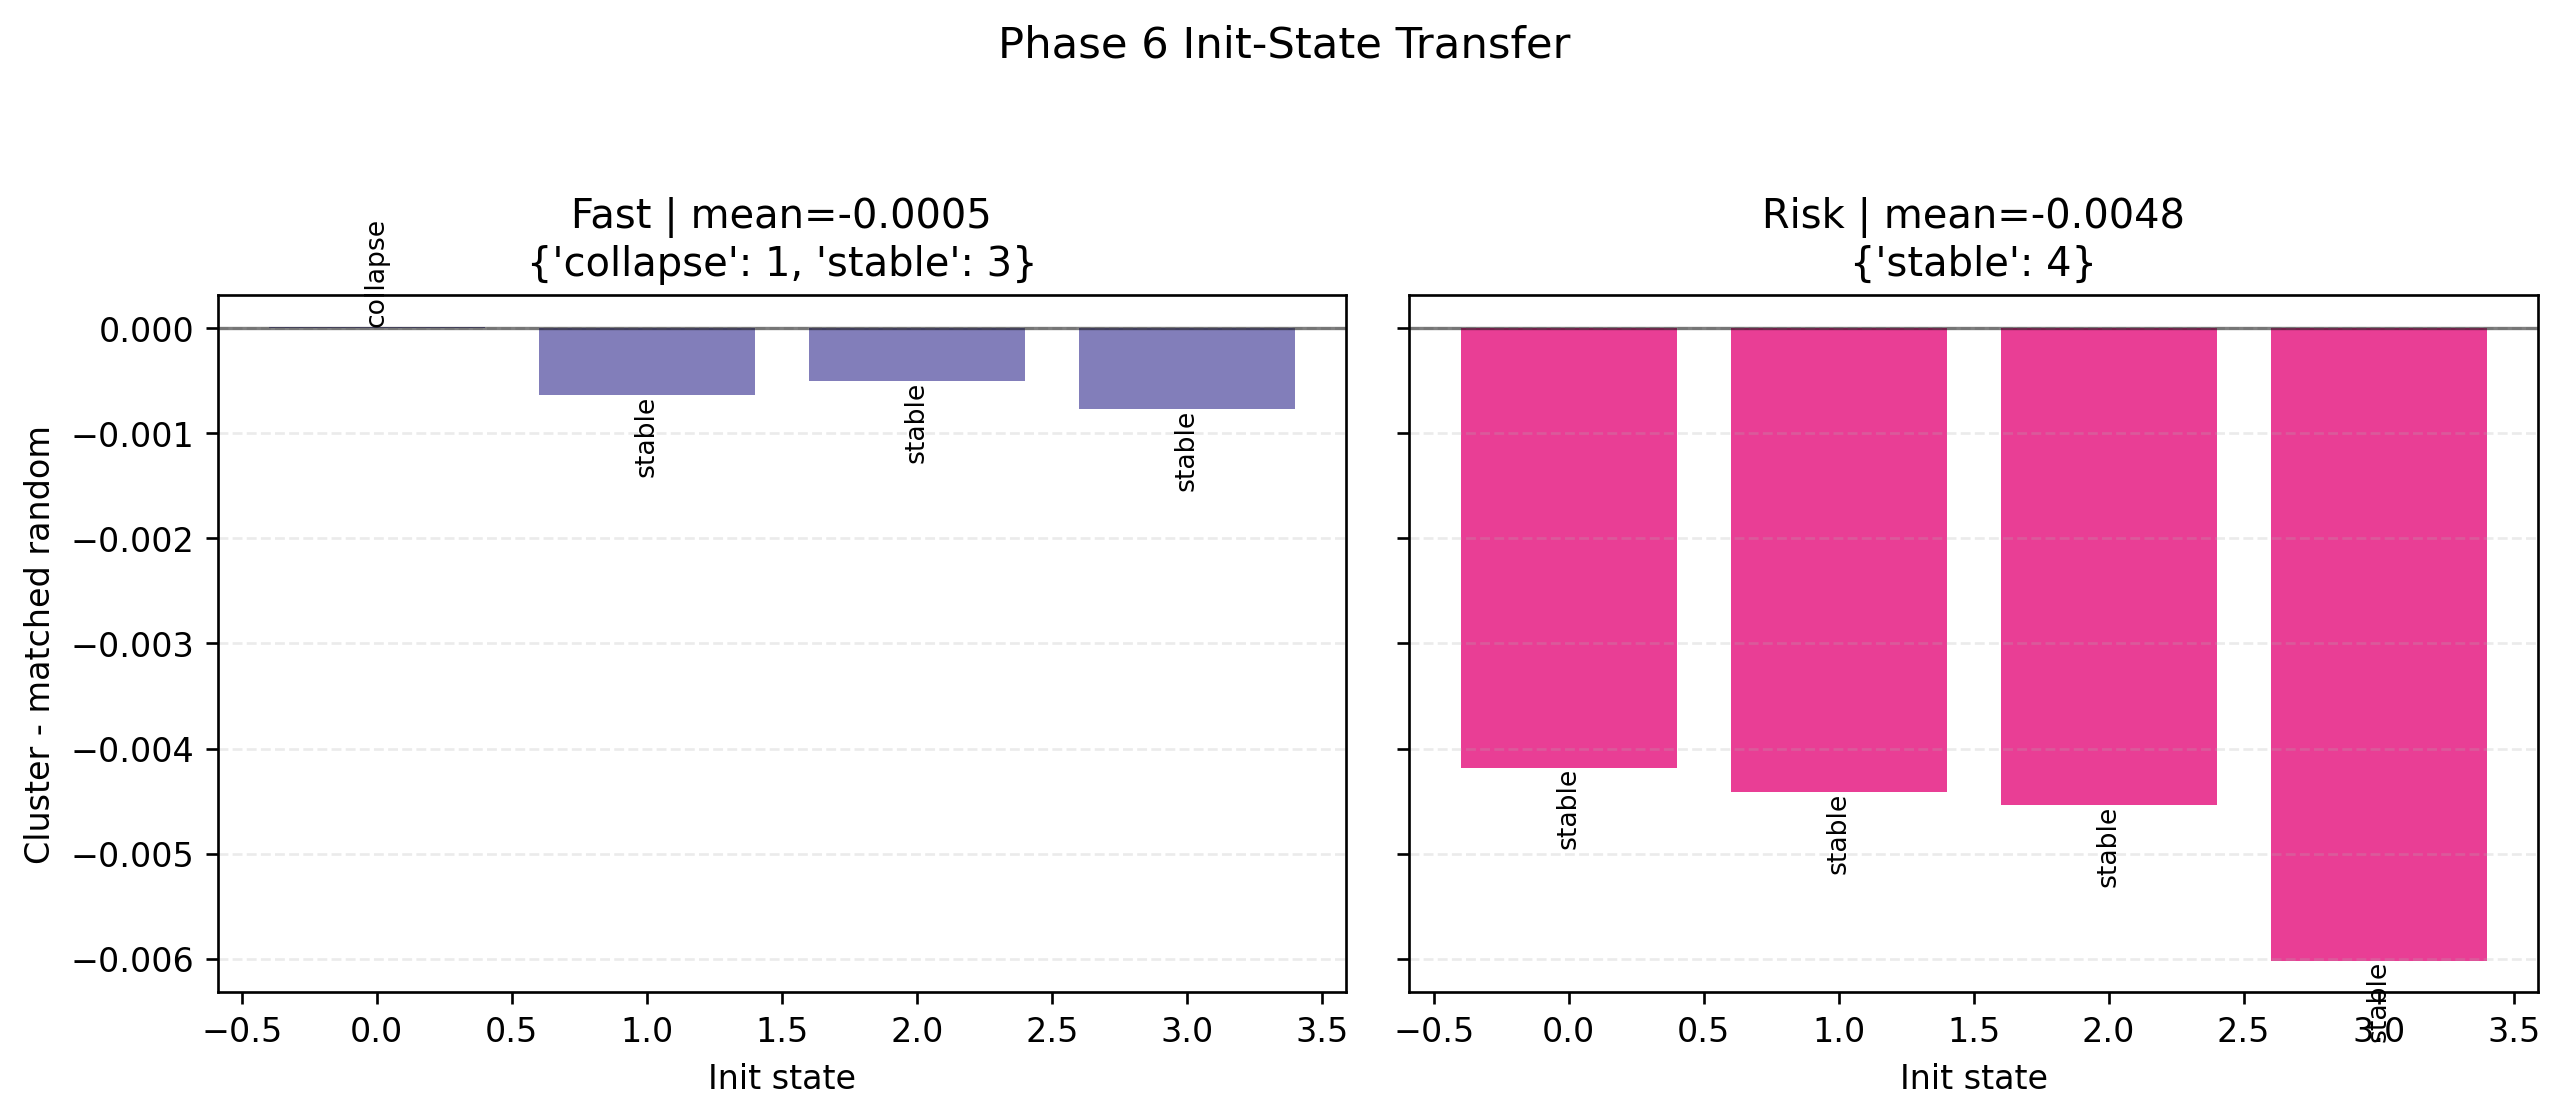
\includegraphics[width=\columnwidth]{plots/report_figure2_init_state_transfer.png}
  \caption{Phase~6 paired init-state transfer. The \texttt{risk} effect remains stable across all fixed visual contexts tested, while \texttt{fast} transfers more weakly.}
  \label{fig:init-transfer}
\end{figure}

\subsection{Transfer under nuisance perturbations}

Phase~7 extends the transfer test to nuisance perturbations. Under a mild primary-camera brightness shift, both \texttt{risk} and \texttt{fast} remained stable overall. Under occlusion, both still transferred, but \texttt{fast} weakened while \texttt{risk} stayed stable and slightly strengthened.

For perturbation analysis, we compare the clean and perturbed effects directly. If $\Delta^{\text{clean}}$ is the clean cluster-vs-random effect and $\Delta^{\text{pert}}$ is the perturbed one, then the effect shift is
\begin{equation}
\delta = \Delta^{\text{pert}} - \Delta^{\text{clean}}.
\label{eq:effect-shift}
\end{equation}
This lets us ask whether the semantic steering effect is preserved under visual corruption, not just whether overall behavior changes.

The strongest summary is:
\begin{itemize}
    \item \texttt{risk}: stable across init states, brightness, and occlusion
    \item \texttt{fast}: stable overall, but weaker and more fragile
\end{itemize}

\begin{figure}[t]
  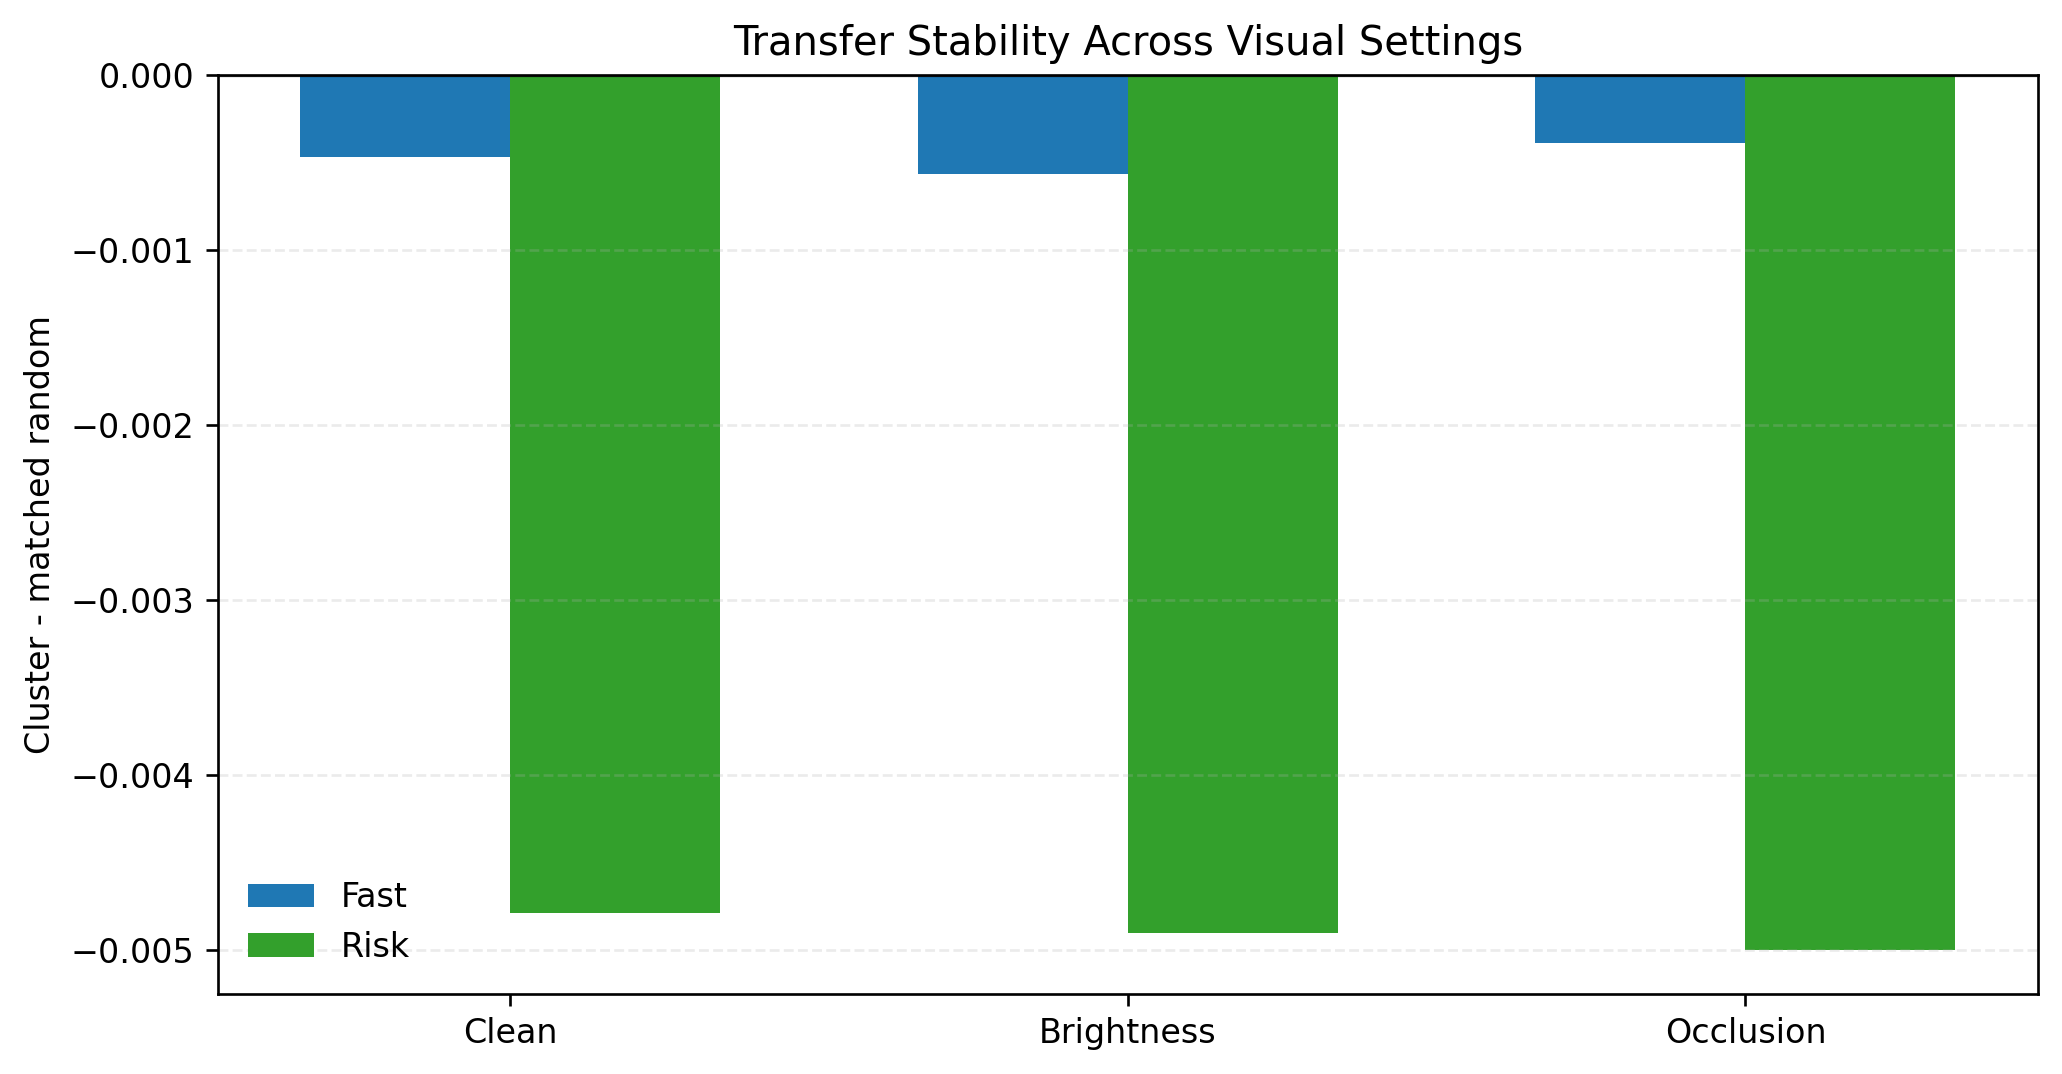
\includegraphics[width=\columnwidth]{plots/report_figure3_transfer_stability.png}
  \caption{Transfer stability across clean, brightness, and occlusion settings. The \texttt{risk} cluster remains robust across all tested perturbations, while \texttt{fast} shows smaller and more fragile effects.}
  \label{fig:transfer-stability}
\end{figure}

\subsection{Error analysis and qualitative examples}

Table~\ref{tab:qualitative-tokens} shows representative decoded token previews from the strongest \texttt{fast} and \texttt{risk} concept candidates. The \texttt{risk} candidate is semantically cleaner: its top decoded tokens are tightly concentrated around \texttt{risk}-related vocabulary, while the \texttt{fast} candidate includes a broader neighborhood of speed-related but more heterogeneous tokens. This is consistent with the stronger and more stable behavior of the \texttt{risk} cluster.

Our clearest qualitative failure case is the \texttt{fast} init-state transfer setting for init state 0. There, the cluster-minus-random effect is approximately $+1.3 \times 10^{-5}$, effectively zero, and the context is classified as a collapse. This illustrates that weak semantic clusters can be real on average while still failing to transfer cleanly in specific visual contexts.

\begin{table}[t]
  \centering
  \scriptsize
  \setlength{\tabcolsep}{3pt}
  \begin{tabular}{p{0.14\columnwidth}p{0.74\columnwidth}}
    \toprule
    Concept & Representative decoded tokens \\
    \midrule
    Fast & \texttt{speed}, \texttt{rapid}, \texttt{speed}, \texttt{fast}, \texttt{Speed}, \texttt{faster}, \texttt{quick}, \texttt{speedy}, \texttt{quick}, \texttt{speeds} \\
    Risk & \texttt{risk}, \texttt{risk}, \texttt{Risk}, \texttt{risks}, \texttt{risked}, \texttt{Risk}, \texttt{risking}, \texttt{Risks}, \texttt{threat}, \texttt{danger} \\
    \bottomrule
  \end{tabular}
  \caption{Representative top decoded token previews for the strongest \texttt{fast} and \texttt{risk} concept candidates used to seed semantic clustering.}
  \label{tab:qualitative-tokens}
\end{table}

\section{Discussion}

The main scientific takeaway is that some mechanistic steering directions in SmolVLA are portable across changing visual contexts. The \texttt{risk} cluster is the clearest example: it consistently outperforms matched random controls and preserves its behavioral effect across paired init states and nuisance perturbations. In that sense, our results support the broader interpretability-and-control picture proposed by \citet{haon2025mechanistic}, while also showing that transfer robustness is cluster-dependent in a continuous-action VLA.

This matters for understanding multimodal policies. If a direction continues to have a similar causal effect even when visual context changes, that suggests the direction is not merely memorizing one scene layout. Instead, it behaves more like a reusable internal feature whose semantics survive interaction with changing visual evidence. Such results can help guide future fine-tuning, debugging, and mechanistic analysis by identifying which internal features are stable enough to matter across environments.

At the same time, our results caution against overly broad claims. Concept labels are operational rather than perfect semantic ground truth. They arise from token-space decoding and clustering, not from a perfect disentanglement of internal representations. This is especially important for weaker concepts. In our case, \texttt{fast} does not literally make the arm move faster in the intuitive sense; instead, it reduces mean displacement relative to its matched random control. For that reason, our strongest claim is about consistent causal influence rather than literal natural-language semantics.

There is also a dual-use aspect to this kind of robustness. The same portability that makes an internal direction scientifically interesting and practically useful for controllability can also make it a safety concern. If a small internal intervention reliably alters behavior across environments, then activation-level control could become a powerful lever for both desirable steering and undesirable manipulation. For this reason, transfer should be interpreted as both an opportunity for interpretability and a reason to think carefully about safeguards.

\section*{Limitations}

This project is still narrower than a full benchmark-scale reproduction. The main limitations are:
\begin{itemize}
    \item \textbf{Single-task scope.} Most quantitative results in this draft come from one LIBERO task \citep{liu2023libero}, so broader task generality remains to be tested.
    \item \textbf{Modest rollout count.} Our rollout counts are intentionally small in order to make the transfer analysis tractable, which limits statistical power for weak effects such as \texttt{fast}.
    \item \textbf{Simulation only.} All conclusions here are based on LIBERO simulation, not real-robot deployment.
    \item \textbf{Backbone-only intervention.} We intervene in the SmolVLA backbone FFNs, not equally across the full downstream action expert, so our evidence is strongest for backbone-to-behavior influence rather than full-policy disentanglement.
\end{itemize}

There is also an architectural limitation. SmolVLA is a continuous-action VLM-plus-expert model rather than an action-token VLA, so our strongest evidence is not direct action-token steering but causal changes in rollout behavior.

\section{Ethical Considerations}

Mechanistic steering is dual-use. The same portability that makes a direction scientifically interesting and potentially useful for fine-tuning or debugging can also make it a powerful intervention lever for changing behavior across environments. Robust activation-level controls therefore raise both interpretability opportunities and misuse risks.

Our semantic labels are operational labels derived from token decoding and clustering, not perfect ground-truth concepts. As our \texttt{fast} example shows, a label that sounds intuitive can correspond to a more complicated behavioral effect in practice. Users could be misled if they assume that an internal cluster named with a familiar word literally enacts that behavior under all conditions.

Finally, all claims in this paper are simulation-only. We do not claim that these steering directions would transfer safely, reliably, or desirably to real robots without additional validation, robustness checks, and human oversight.

\section{Conclusion}

We adapted a value-vector steering framework \citep{haon2025mechanistic} to SmolVLA \citep{shukor2025smolvla} and used it to study whether internal steering effects transfer across visual contexts. Our pipeline extracts all FFN value vectors, assigns approximate semantics through token decoding and clustering, intervenes at the correct pre-\texttt{down\_proj} hook point, and evaluates concept-aligned clusters against matched random controls.

The strongest result is that the \texttt{risk} cluster produces a robust causal effect that transfers across fixed visual contexts, brightness perturbations, and occlusion. The \texttt{fast} cluster also transfers, but more weakly. These results provide evidence that at least some internal control directions in a vision-language-action model are portable rather than purely scene-specific artifacts.

\section*{Acknowledgments}

This project was developed as a course research effort on mechanistic interpretability for vision-language-action models, with SmolVLA used as the main case study.

\bibliography{custom}

\end{document}
